% ---------
%  Compile with "pdflatex hw0".
% --------
%!TEX TS-program = pdflatex
%!TEX encoding = UTF-8 Unicode

\documentclass[11pt]{article}
\usepackage{jeffe,handout,graphicx}
\usepackage[utf8]{inputenc}		% Allow some non-ASCII Unicode in source
\usepackage{tikz}

% =========================================================
%   Define common stuff for solution headers
% =========================================================
\Class{CS/ECE 374}
\Semester{Spring 2023}
\Authors{1}
\AuthorOne{William Cheng}{shihuac2@illinois.edu}
%\Section{}

% =========================================================
\begin{document}

% ---------------------------------------------------------


\HomeworkHeader{2}{1}	% homework number, problem number

\begin{solution} 
\begin{enumerate}[(a)]

\item $(0+1)^{*}111(0+1)^{*}10 + (0+1)^{*}1110$. \\
	\emph{Explanation.} There are two cases: 1) the $1$ in the ending $10$ is a part of the substring $111$, which can be represented as $(0+1)^{*}1110$; 2) the $1$ in the ending $10$ is not a part of the substring $111$, which can be represented as $(0+1)^{*}111(0+1)^{*}10$. The desired expression is the union of these two expressions. 
\item $1^{*}0^{*}1^{*}$. \\
	\emph{Explanation.} Consider a string that does not contain the subsequence $010$. Then it contains at most one block of $0$'s otherwise it must contain the subsequence $010$ since there must be at least a $1$ between two blocks of $0$'s. $1^{*}0^{*}1^{*}$ represents all such strings.
\item $0^{*}(10^{*}+10^{*}10^{*})(10^{*}10^{*}10^{*})^{*}$.\\
	\emph{Explanation.} There are two cases: 1) $\#1's$ mod $3 = 1$; 2) $\#1's$ mod $3 = 2$. The $(10^{*}10^{*}10^{*})^{*}$ part accounts for multiples of $3$ of $1$'s. The part before it accounts for both cases, either containing one $1$ or two $1$'s.
\item $w_{1}+w_{2}+...+w_{k}$.\\
	\emph{Explanation.} The expression represents the union of all $\{ w_{i} \}$ where $w_{i}\in L$, which is $L$ itself.
\item Let $Q=\{ x\in \Sigma^{*} \text{ }| \text{ } \lvert x \rvert \leq h  \} \setminus L=\{q_{1},q_{2},...,q_{m}\}$. Then $Q$ is finite since $h$ is a finite number. The desired expression is:\\\\
	$q_{1}+q_{2}+...+q_{m}+\underbrace{(0+1)(0+1)...(0+1)}_{h+1}(0+1)^{*}$.\\\\
	\emph{Explanation.} All strings with length $>h$ are automatically in $\bar{L}$ since the longest string in $L$ has length $h$. The desired expression is the union of all strings with length $>h$ and all strings with length $\leq$ h that are not in $L$.

\end{enumerate}
\end{solution}

% ---------------------------------------------------------
\HomeworkHeader{2}{2}

\begin{solution}
\begin{enumerate}[(a)]
\item The DFA is shown below.
\begin{center}
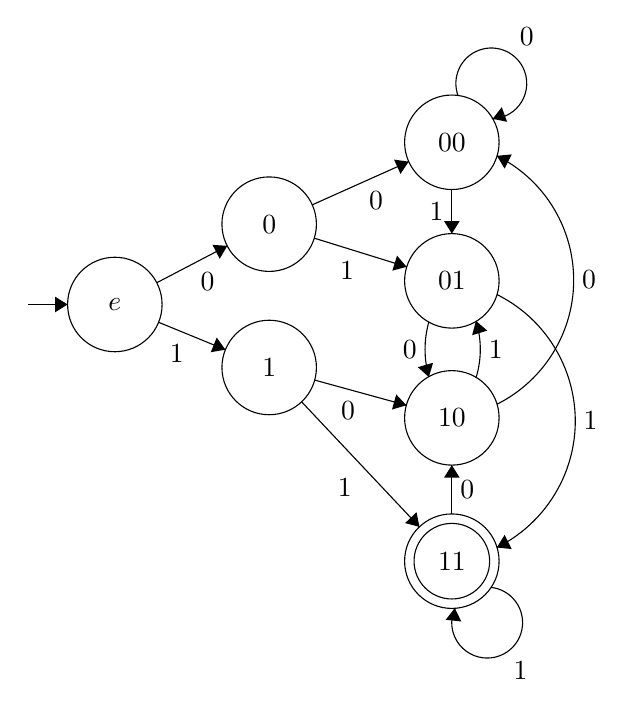
\begin{tikzpicture}[scale=0.2]
\tikzstyle{every node}+=[inner sep=0pt]
\draw [black] (16.1,-19.7) circle (3);
\draw (16.1,-19.7) node {$e$};
\draw [black] (25.9,-14.6) circle (3);
\draw (25.9,-14.6) node {$0$};
\draw [black] (25.9,-23.7) circle (3);
\draw (25.9,-23.7) node {$1$};
\draw [black] (37.5,-9.4) circle (3);
\draw (37.5,-9.4) node {$00$};
\draw [black] (37.5,-18.2) circle (3);
\draw (37.5,-18.2) node {$01$};
\draw [black] (37.5,-26.9) circle (3);
\draw (37.5,-26.9) node {$10$};
\draw [black] (37.5,-36) circle (3);
\draw (37.5,-36) node {$11$};
\draw [black] (37.5,-36) circle (2.4);
\draw [black] (18.76,-18.32) -- (23.24,-15.98);
\fill [black] (23.24,-15.98) -- (22.3,-15.91) -- (22.76,-16.8);
\draw (21.99,-17.65) node [below] {$0$};
\draw [black] (18.88,-20.83) -- (23.12,-22.57);
\fill [black] (23.12,-22.57) -- (22.57,-21.8) -- (22.19,-22.73);
\draw (20.04,-22.22) node [below] {$1$};
\draw [black] (28.79,-24.5) -- (34.61,-26.1);
\fill [black] (34.61,-26.1) -- (33.97,-25.41) -- (33.7,-26.37);
\draw (30.91,-25.86) node [below] {$0$};
\draw [black] (27.96,-25.88) -- (35.44,-33.82);
\fill [black] (35.44,-33.82) -- (35.26,-32.89) -- (34.53,-33.58);
\draw (31.17,-31.32) node [left] {$1$};
\draw [black] (28.77,-15.49) -- (34.63,-17.31);
\fill [black] (34.63,-17.31) -- (34.02,-16.6) -- (33.72,-17.55);
\draw (30.84,-16.94) node [below] {$1$};
\draw [black] (28.64,-13.37) -- (34.76,-10.63);
\fill [black] (34.76,-10.63) -- (33.83,-10.5) -- (34.24,-11.41);
\draw (32.68,-12.51) node [below] {$0$};
\draw [black] (37.894,-6.438) arc (200.15622:-87.84378:2.25);
\draw (42.26,-3.29) node [above] {$0$};
\fill [black] (40.09,-7.91) -- (41.01,-8.1) -- (40.67,-7.17);
\draw [black] (37.5,-12.4) -- (37.5,-15.2);
\fill [black] (37.5,-15.2) -- (38,-14.4) -- (37,-14.4);
\draw (37,-13.8) node [left] {$1$};
\draw [black] (36.044,-24.308) arc (-164.0827:-195.9173:6.411);
\fill [black] (36.04,-24.31) -- (36.31,-23.4) -- (35.34,-23.68);
\draw (35.3,-22.55) node [left] {$0$};
\draw [black] (40.358,-19.066) arc (63.56505:-63.56505:8.972);
\fill [black] (40.36,-35.13) -- (41.3,-35.23) -- (40.85,-34.33);
\draw (45.84,-27.1) node [right] {$1$};
\draw [black] (40.358,-10.263) arc (63.45929:-63.45929:8.817);
\fill [black] (40.36,-10.26) -- (40.85,-11.07) -- (41.3,-10.17);
\draw (45.74,-18.15) node [right] {$0$};
\draw [black] (39.035,-20.743) arc (17.11705:-17.11705:6.14);
\fill [black] (39.03,-20.74) -- (38.79,-21.65) -- (39.75,-21.36);
\draw (39.81,-22.55) node [right] {$1$};
\draw [black] (39.982,-37.664) arc (83.89184:-204.10816:2.25);
\draw (41.86,-42.35) node [below] {$1$};
\fill [black] (37.69,-38.98) -- (37.11,-39.72) -- (38.1,-39.83);
\draw [black] (37.5,-33) -- (37.5,-29.9);
\fill [black] (37.5,-29.9) -- (37,-30.7) -- (38,-30.7);
\draw (38,-31.45) node [right] {$0$};
\draw [black] (10.6,-19.7) -- (13.1,-19.7);
\fill [black] (13.1,-19.7) -- (12.3,-19.2) -- (12.3,-20.2);
\end{tikzpicture}
\end{center}

The meaning of each state is that the name of each state represents the last two letters of the current longest prefix being read from the input string. Therefore, when the whole input string is read, the state of the DFA represents the last two letters of the input string. The only accepting state is $11$.

\item The DFA is shown below.
\begin{center}
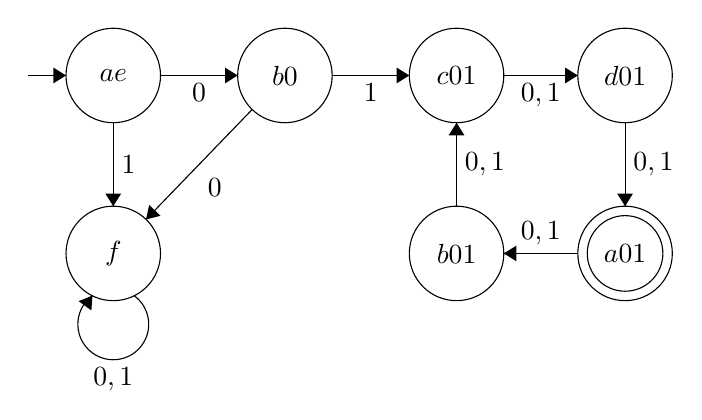
\begin{tikzpicture}[scale=0.2]
\tikzstyle{every node}+=[inner sep=0pt]
\draw [black] (12.1,-17.6) circle (3);
\draw (12.1,-17.6) node {$ae$};
\draw [black] (44.6,-28.9) circle (3);
\draw (44.6,-28.9) node {$a01$};
\draw [black] (44.6,-28.9) circle (2.4);
\draw [black] (23,-17.6) circle (3);
\draw (23,-17.6) node {$b0$};
\draw [black] (33.9,-28.9) circle (3);
\draw (33.9,-28.9) node {$b01$};
\draw [black] (33.9,-17.6) circle (3);
\draw (33.9,-17.6) node {$c01$};
\draw [black] (44.6,-17.6) circle (3);
\draw (44.6,-17.6) node {$d01$};
\draw [black] (12.1,-28.9) circle (3);
\draw (12.1,-28.9) node {$f$};
\draw [black] (6.7,-17.6) -- (9.1,-17.6);
\fill [black] (9.1,-17.6) -- (8.3,-17.1) -- (8.3,-18.1);
\draw [black] (12.1,-20.6) -- (12.1,-25.9);
\fill [black] (12.1,-25.9) -- (12.6,-25.1) -- (11.6,-25.1);
\draw (12.6,-23.25) node [right] {$1$};
\draw [black] (15.1,-17.6) -- (20,-17.6);
\fill [black] (20,-17.6) -- (19.2,-17.1) -- (19.2,-18.1);
\draw (17.55,-18.1) node [below] {$0$};
\draw [black] (13.423,-31.58) arc (54:-234:2.25);
\draw (12.1,-36.15) node [below] {$0,1$};
\fill [black] (10.78,-31.58) -- (9.9,-31.93) -- (10.71,-32.52);
\draw [black] (26,-17.6) -- (30.9,-17.6);
\fill [black] (30.9,-17.6) -- (30.1,-17.1) -- (30.1,-18.1);
\draw (28.45,-18.1) node [below] {$1$};
\draw [black] (20.92,-19.76) -- (14.18,-26.74);
\fill [black] (14.18,-26.74) -- (15.1,-26.51) -- (14.38,-25.82);
\draw (18.08,-24.72) node [right] {$0$};
\draw [black] (36.9,-17.6) -- (41.6,-17.6);
\fill [black] (41.6,-17.6) -- (40.8,-17.1) -- (40.8,-18.1);
\draw (39.25,-18.1) node [below] {$0,1$};
\draw [black] (44.6,-20.6) -- (44.6,-25.9);
\fill [black] (44.6,-25.9) -- (45.1,-25.1) -- (44.1,-25.1);
\draw (45.1,-23.25) node [right] {$0,1$};
\draw [black] (41.6,-28.9) -- (36.9,-28.9);
\fill [black] (36.9,-28.9) -- (37.7,-29.4) -- (37.7,-28.4);
\draw (39.25,-28.4) node [above] {$0,1$};
\draw [black] (33.9,-25.9) -- (33.9,-20.6);
\fill [black] (33.9,-20.6) -- (33.4,-21.4) -- (34.4,-21.4);
\draw (34.4,-23.25) node [right] {$0,1$};
\end{tikzpicture}
\end{center}
\begin{itemize}
\item $ae$: the current prefix is $\epsilon$
\item $b0$: the current prefix is $0$
\item $f$: the input string fails to start with $01$
\item $c01$: the input string starts with $01$, and the current length is $2$ mod $4$
\item $d01$: the input string starts with $01$, and the current length is $3$ mod $4$
\item $a01$: the input string starts with $01$, and the current length is $0$ mod $4$
\item $b01$: the input string starts with $01$, and the current length is $1$ mod $4$
\end{itemize}

\item The DFA is shown below.
\begin{center}
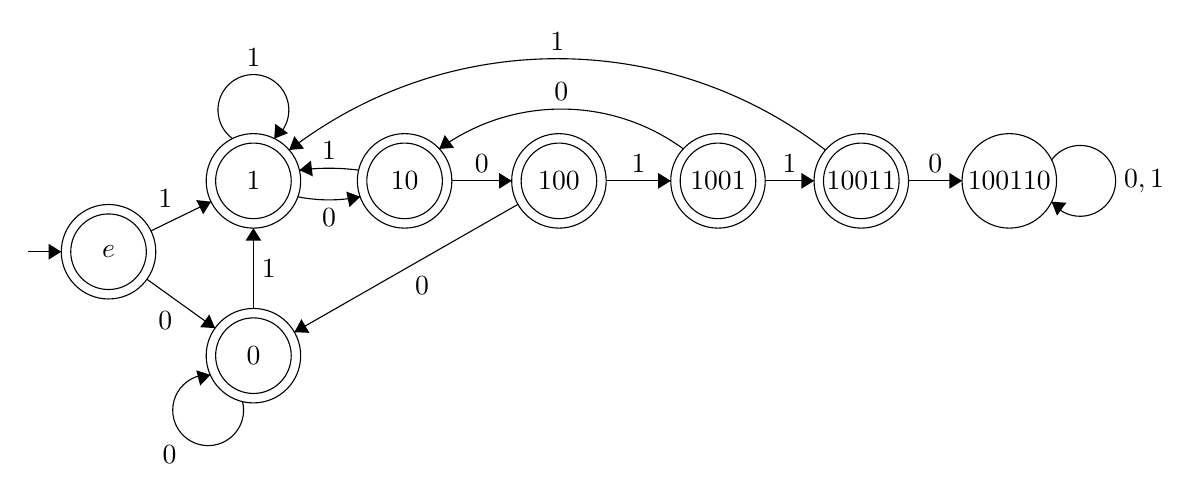
\begin{tikzpicture}[scale=0.2]
\tikzstyle{every node}+=[inner sep=0pt]
\draw [black] (12.4,-16.4) circle (3);
\draw (12.4,-16.4) node {$e$};
\draw [black] (12.4,-16.4) circle (2.4);
\draw [black] (21.6,-11.9) circle (3);
\draw (21.6,-11.9) node {$1$};
\draw [black] (21.6,-11.9) circle (2.4);
\draw [black] (21.6,-23) circle (3);
\draw (21.6,-23) node {$0$};
\draw [black] (21.6,-23) circle (2.4);
\draw [black] (31.2,-11.9) circle (3);
\draw (31.2,-11.9) node {$10$};
\draw [black] (31.2,-11.9) circle (2.4);
\draw [black] (41,-11.9) circle (3);
\draw (41,-11.9) node {$100$};
\draw [black] (41,-11.9) circle (2.4);
\draw [black] (51.1,-11.9) circle (3);
\draw (51.1,-11.9) node {$1001$};
\draw [black] (51.1,-11.9) circle (2.4);
\draw [black] (60.2,-11.9) circle (3);
\draw (60.2,-11.9) node {$10011$};
\draw [black] (60.2,-11.9) circle (2.4);
\draw [black] (69.6,-11.9) circle (3);
\draw (69.6,-11.9) node {$100110$};
\draw [black] (72.28,-10.577) arc (144:-144:2.25);
\draw (76.85,-11.9) node [right] {$0,1$};
\fill [black] (72.28,-13.22) -- (72.63,-14.1) -- (73.22,-13.29);
\draw [black] (15.09,-15.08) -- (18.91,-13.22);
\fill [black] (18.91,-13.22) -- (17.97,-13.12) -- (18.41,-14.02);
\draw (16.01,-13.64) node [above] {$1$};
\draw [black] (14.84,-18.15) -- (19.16,-21.25);
\fill [black] (19.16,-21.25) -- (18.8,-20.38) -- (18.22,-21.19);
\draw (16,-20.2) node [below] {$0$};
\draw [black] (28.387,-12.911) arc (-78.69963:-101.30037:10.141);
\fill [black] (28.39,-12.91) -- (27.5,-12.58) -- (27.7,-13.56);
\draw (26.4,-13.61) node [below] {$0$};
\draw [black] (20.277,-9.22) arc (234:-54:2.25);
\draw (21.6,-4.65) node [above] {$1$};
\fill [black] (22.92,-9.22) -- (23.8,-8.87) -- (22.99,-8.28);
\draw [black] (24.516,-11.218) arc (97.33962:82.66038:14.747);
\fill [black] (24.52,-11.22) -- (25.37,-11.61) -- (25.25,-10.62);
\draw (26.4,-10.6) node [above] {$1$};
\draw [black] (21.6,-20) -- (21.6,-14.9);
\fill [black] (21.6,-14.9) -- (21.1,-15.7) -- (22.1,-15.7);
\draw (22.1,-17.45) node [right] {$1$};
\draw [black] (20.905,-25.906) arc (14.28574:-273.71426:2.25);
\draw (16.28,-28.69) node [below] {$0$};
\fill [black] (18.87,-24.22) -- (17.97,-23.93) -- (18.22,-24.9);
\draw [black] (34.2,-11.9) -- (38,-11.9);
\fill [black] (38,-11.9) -- (37.2,-11.4) -- (37.2,-12.4);
\draw (36.1,-11.4) node [above] {$0$};
\draw [black] (44,-11.9) -- (48.1,-11.9);
\fill [black] (48.1,-11.9) -- (47.3,-11.4) -- (47.3,-12.4);
\draw (46.05,-11.4) node [above] {$1$};
\draw [black] (38.4,-13.39) -- (24.2,-21.51);
\fill [black] (24.2,-21.51) -- (25.15,-21.55) -- (24.65,-20.68);
\draw (32.3,-17.95) node [below] {$0$};
\draw [black] (54.1,-11.9) -- (57.2,-11.9);
\fill [black] (57.2,-11.9) -- (56.4,-11.4) -- (56.4,-12.4);
\draw (55.65,-11.4) node [above] {$1$};
\draw [black] (33.4,-9.87) arc (126.16495:53.83505:13.134);
\fill [black] (33.4,-9.87) -- (34.34,-9.8) -- (33.75,-8.99);
\draw (41.15,-6.84) node [above] {$0$};
\draw [black] (23.872,-9.944) arc (127.64131:52.35869:27.881);
\fill [black] (23.87,-9.94) -- (24.81,-9.85) -- (24.2,-9.06);
\draw (40.9,-3.64) node [above] {$1$};
\draw [black] (63.2,-11.9) -- (66.6,-11.9);
\fill [black] (66.6,-11.9) -- (65.8,-11.4) -- (65.8,-12.4);
\draw (64.9,-11.4) node [above] {$0$};
\draw [black] (7.3,-16.4) -- (9.4,-16.4);
\fill [black] (9.4,-16.4) -- (8.6,-15.9) -- (8.6,-16.9);
\end{tikzpicture}
\end{center}
The meaning of each state is the last letter(s) of the current longest prefix of the input string. Every state except $100110$ is an accepting state, so that when $100110$ is a substring, the DFA would not reach an accepting state and the input string will therefore not be accepted. Otherwise, the input string will always be accepted.

\item $M=(Q,\Sigma,\delta,s,A)$ where
\begin{itemize}
\item $Q=\{\epsilon, a_{1}, a_{1}a_{2}, ......, a_{1}a_{2}...a_{k-1}, a_{1}a_{2}...a_{k}\}$
\item $\Sigma=\{ 0,1 \}$
\item $\delta=(a_{1}a_{2}...a_{m}, a_{n})\to$
\begin{math}
  \left\{
    \begin{array}{ll}
      	a_{1}a_{2}...a_{m}a_{m+1} &\text{$a_{n}=a_{m+1},m<k$}\\
      	a_{1}a_{2}...a_{k} &\text{$m=k$}\\
		a_{i}...a_{m}a_{n}=a_{1}a_{2}...a_{m-i} &\text{$a_{n}\neq a_{m+1}$, $i$ is the smallest index possible}\\
		\epsilon &\text{$a_{n}\neq a_{m+1}$, no suffix matching prefix of $s$}
    \end{array}
  \right.
\end{math}\\
$(\epsilon, a_{n})\to$
\begin{math}
  \left\{
    \begin{array}{ll}
      	a_{1} &\text{$a_{n}=a_{1}$}\\
		\epsilon &\text{$a_{n}\neq a_{1}$}
    \end{array}
  \right.
\end{math}\\
\item $s=\epsilon$
\item $A=\{ a_{1}a_{2}...a_{k} \}$
\end{itemize}
The DFA has $k+1$ states.

\item $M=(Q,\Sigma_M, \delta, s, A)$ where
\begin{itemize}
\item $Q=\{ (q_1, q_2, q_3, q_4)$ | $q_1\in Q_1, q_2\in Q_2, q_3\in Q_3, q_4\in Q_4 \}$
\item $\Sigma_M = \Sigma$
\item $\delta((q_1,q_2,q_3,q_4), a)=(\delta_1(q_1,a), \delta_2(q_2,a), \delta_3(q_3,a), \delta_4(q_4,a))$
\item $s=(s_1, s_2, s_3, s_4)$
\item $A=$\\\\
\begin{math}
    \begin{array}{ll}
      	\{ (a_1, a_2, a_3, a_4) &\text{ | } 
			(a_1\in A_1 \text{ and } a_2\notin A_2 \text{ and } a_3\notin A_3 \text{ and } a_4\notin A_4)\\
			&\text{or } (a_1\notin A_1 \text{ and } a_2\in A_2 \text{ and } a_3\notin A_3 \text{ and } a_4\notin A_4)\\
			&\text{or } (a_1\notin A_1 \text{ and } a_2\notin A_2 \text{ and } a_3\in A_3 \text{ and } a_4\notin A_4)\\
			&\text{or } (a_1\notin A_1 \text{ and } a_2\notin A_2 \text{ and } a_3\notin A_3 \text{ and } a_4\in A_4)
		\}
    \end{array}
\end{math}\\
\end{itemize}
\end{enumerate}
\end{solution}




\end{document}
